\subsection{Glaciares}

Los glaciares son estructuras complejas constituidas por hielo, nieve, agua, rocas y sedimentos, que se desplazan bajo la acción de la gravedad y de su propia masa \cite{cuffey2010physics}. Estos se originan en regiones donde la acumulación de nieve supera a la ablación, es decir, la pérdida de masa debido a procesos como la fusión y la sublimación \cite{griggs2002climate}.

En el movimiento de los glaciares intervienen factores internos como la temperatura y la estructura del hielo, y factores externos como la topografía y las condiciones climáticas \cite{benn2010glaciers}. Estos elementos naturales son fundamentales en el balance global del agua dulce y tienen un impacto significativo en el clima y en los ecosistemas \cite{kargel2014global}.

La formación de los glaciares se efectúa mediante la acumulación continua de nieve y hielo en una misma área durante un periodo prolongado, situándose principalmente en regiones de elevada altitud, por encima del nivel de las nieves perpetuas \cite{houghton2001climate}.

\begin{figure}[H]
    \begin{center}
        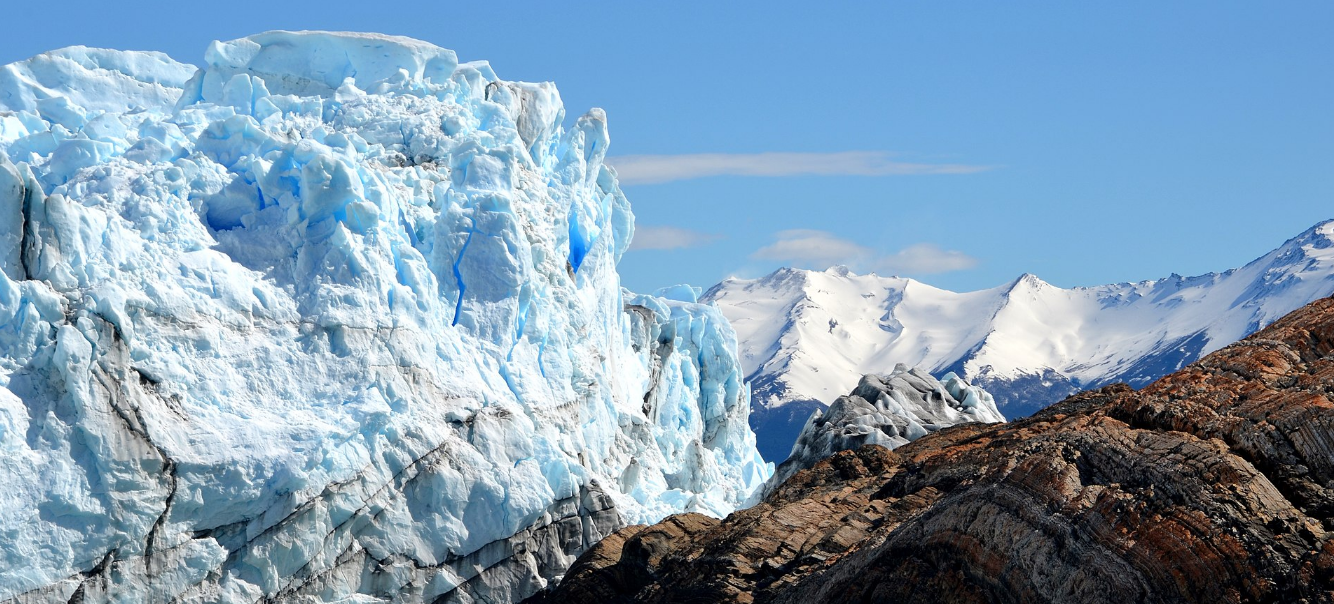
\includegraphics[width=1\textwidth]{Images/GlaciaresFotografia.png}
    \end{center}
    \caption{Fotografía de un glaciar (Glaciar Perito Moreno - Chile)}
    \reference{Datos tomados de \citeA{ermolin2015ambientes}.}
    \label{fig:Glaciar}
\end{figure}

Los glaciares son vitales como reservorios de agua dulce. Según \citeA{ermolin2015ambientes}, sólo el 3\% del agua del planeta es agua dulce. De este porcentaje, el 77\% se halla en la criósfera, región de la corteza terrestre donde predominan las bajas temperaturas y donde el hielo se mantiene durante la mayoría del año \cite{ermolin2015ambientes}. En términos más específicos, el 91\% de las reservas de agua dulce se encuentra en la Antártida, el 8\% en la sabana de Groenlandia y solo el 1\% en los glaciares de montaña continental \cite{benn2010glaciers}. Estos datos subrayan la importancia crítica de la preservación de los glaciares como principales fuentes de agua dulce a nivel global.

\subsubsection{Sistemas glaciares}

Los glaciares se originan debido a la acumulación constante de nieve, proveniente de fenómenos como nevadas, avalanchas, deslizamiento de rocas, por mencionar algunos. Esta acumulación se ve impulsada por condiciones climáticas y topográficas específicas que permiten que la nieve se compacte y forme hielo. Sin embargo, los glaciares no son estáticos; fluyen pendiente abajo impulsados por la fuerza gravitacional de la Tierra. Este movimiento es parte de un delicado equilibrio conocido como balance de masa, que compara las tasas de acumulación y ablación, o pérdida de masa. La ablación puede ocurrir debido a una variedad de factores, como la evaporación y el derretimiento, y se considera que los glaciares están en retroceso cuando la tasa de ablación supera la de acumulación \cite{benn2010glaciers}.

\begin{figure}[H]
    \begin{center}
        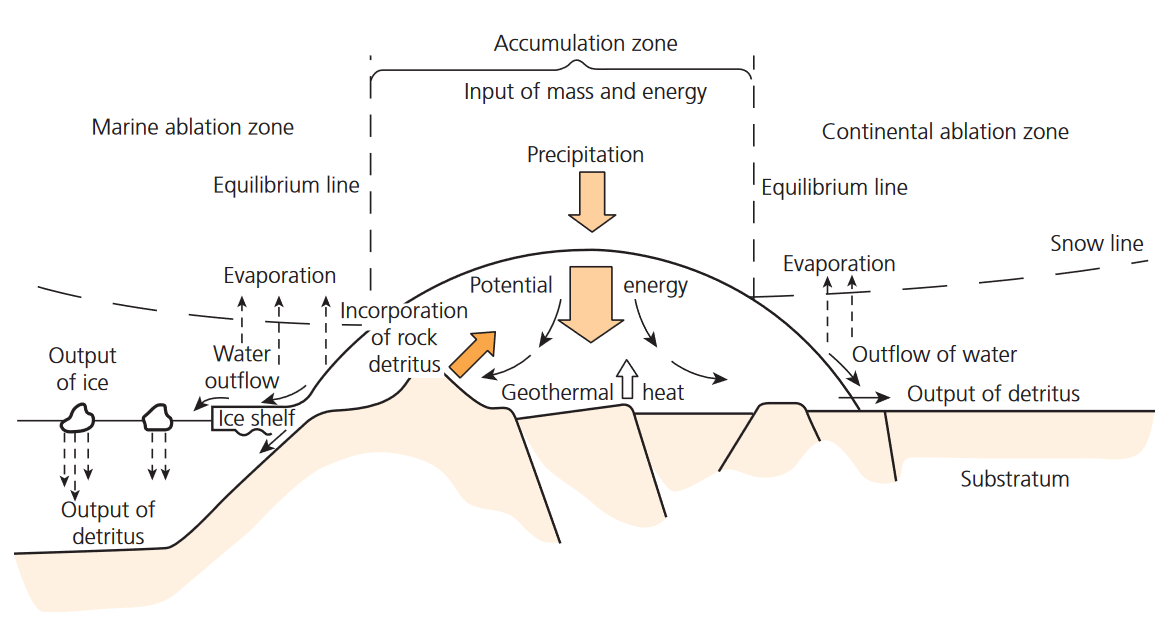
\includegraphics[width=1\textwidth]{Images/Glaciares.png}
    \end{center}
    \caption{Sistemas glaciares}
    \reference{Datos tomados de \citeA{benn2010glaciers}.}
    \label{fig:SistemasGlaciares}
\end{figure}

Factores ambientales como las condiciones atmosféricas y las variaciones térmicas ejercen un impacto directo sobre los glaciares, en particular sobre la altitud de la línea de equilibrio (ELA, por sus siglas en inglés: Equilibrium Line Altitude). La ELA delimita dos regiones diferenciadas en un glaciar: la zona de acumulación y la zona de ablación. En la Figura \ref{fig:SistemasGlaciares}, se observa cómo estas dos zonas se encuentran separadas por la ELA. En la zona de acumulación, la formación de hielo por medio de la acumulación de nieve es predominante sobre el proceso de ablación, es decir, la pérdida de hielo mediante fusión o evaporación. Contrariamente, en la zona de ablación, el proceso de pérdida de hielo es más prominente que el de acumulación  \cite{benn2010glaciers}.

Los glaciares avanzan desde las zonas de acumulación hacia las zonas de ablación a través de deslizamiento y deformación. Este movimiento está regulado por un equilibrio entre las fuerzas que lo impulsan, como la gravedad, y las fuerzas que lo resisten. Cuando están en equilibrio, el flujo del glaciar se mantiene constante \cite{benn2010glaciers, cuffey2010physics}. Sin embargo, factores externos pueden provocar cambios rápidos, como avances o retrocesos. En su trayecto, los glaciares actúan como poderosos agentes erosivos, modelando el paisaje para crear cuencas y fiordos, y eliminando suelo y otros materiales \cite{ermolin2015ambientes}. Además, transportan limo y grava a lo largo de grandes distancias, acumulando estos materiales desde su base hasta el fondo del océano. Dejan un legado de sedimentos y formaciones geográficas, como morrenas y circos, que ofrecen pistas sobre el clima anterior y modifican el terreno, afectando su uso por los seres humanos \cite{benn2010glaciers}.

El agua de deshielo juega un papel esencial, especialmente en la hidrología de las áreas cercanas a los glaciares. Esta agua se incorpora en varios sistemas hídricos, como océanos, ríos y la atmósfera. Participa en un flujo constante entre diferentes reservorios de agua, como océanos, atmósfera, criósfera e hidrosfera, lo que resulta en cambios en el almacenamiento de agua. Por ejemplo, si los glaciares almacenan más agua, el nivel del mar tiende a disminuir y lo contrario ocurre si liberan más agua. Cambios en el volumen del hielo glaciar no solo afectan los niveles del mar, sino también la presión sobre la corteza terrestre y la distribución de la masa global \cite{benn2010glaciers}.

\subsubsection{Partes de un glaciar}

Las partes de un glaciar están estrechamente vinculadas al funcionamiento del sistema glaciar en su conjunto. Según \citeA{inaigem2017manual}, un glaciar se compone de tres partes: la zona de acumulación, la zona de ablación y la altitud de la línea de equilibrio (ELA).

La zona de acumulación corresponde al área donde se acumula la nieve durante un año hidrológico y ofrece datos sobre la cantidad de precipitaciones sólidas en ese periodo. Por otro lado, la zona de ablación es donde predominan los procesos de fusión, evaporación, sublimación y desprendimiento de masas de hielo. La altitud de la línea de equilibrio (ELA) es una línea teórica que separa la zona de acumulación de la zona de ablación \cite{francou2004tropical, benn2010glaciers}.

Como se puede ver en la Figura \ref{fig:PartesGlaciar}, la zona de acumulación y la zona de ablación están separadas por la altitud de la línea de equilibrio (ELA), que representa la zona de equilibrio entre ambas \cite{ideam2012glaciares}.

\begin{figure}[H]
    \begin{center}
        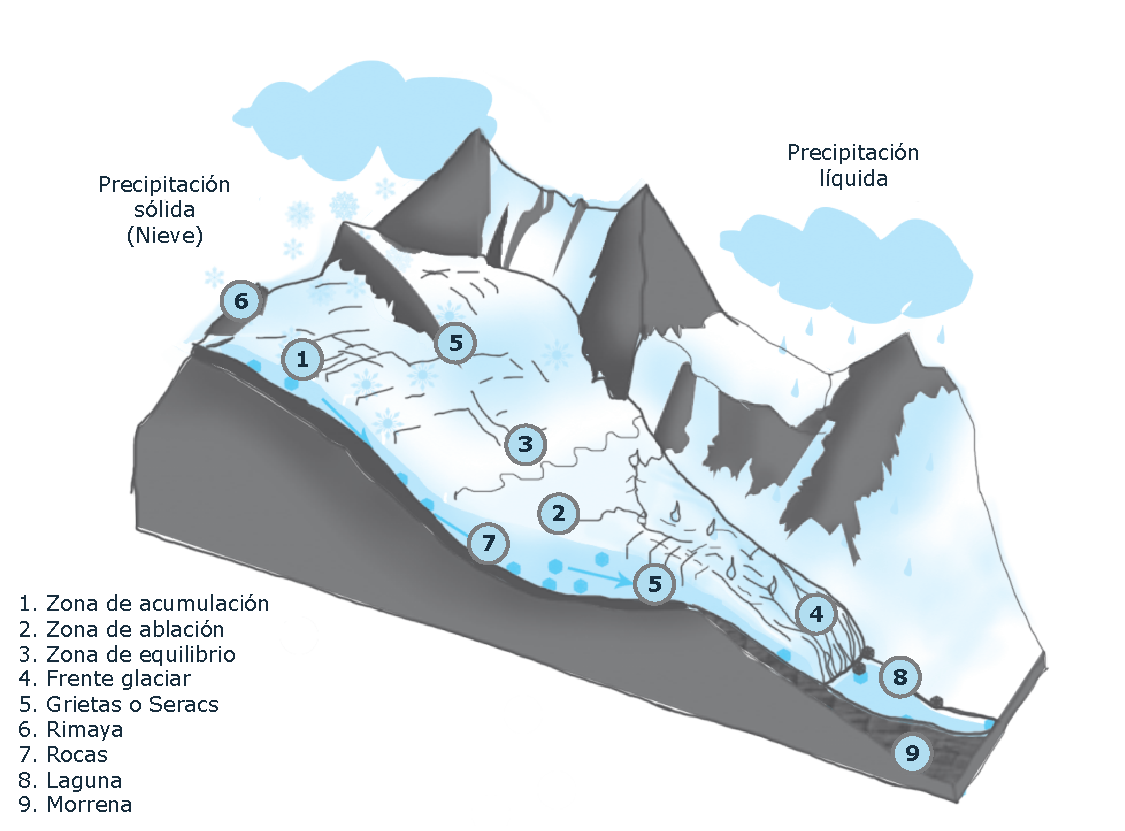
\includegraphics[width=1\textwidth]{Images/PartesGlaciar.pdf}
    \end{center}
    \caption{Partes de un glaciar.}
    \reference{Datos extraídos de \citeA{ideam2012glaciares}.}
    \label{fig:PartesGlaciar}
\end{figure}

En la zona de acumulación, es común encontrar distintos tipos de grietas, como Rimabas y Seracs. Esta área es susceptible a avalanchas debido a las zonas de desprendimiento que pueden extenderse hasta la zona de ablación. Por su parte, la zona de ablación se caracteriza por la presencia de sedimentos y formaciones geográficas como morrenas y circos, así como frentes glaciares, que son aún más propensos a desprendimientos y avalanchas. Además, en esta zona es posible encontrar lagunas de origen glaciar, que son el destino de las aguas de deshielo. Dependiendo de su ubicación, estas aguas pueden dar origen a ríos o desembocar directamente en el mar.

\subsubsection{Clasificación de los glaciares}

La clasificación de los glaciares se determina generalmente por diversos factores, que pueden abarcar la morfología, el tamaño, la dinámica, la temperatura, y el contenido de impurezas en el glaciar. Estas características dan lugar a una amplia clasificación que, según la información recopilada por instituciones especializadas de la región como el Instituto Nacional de Investigación en Glaciares y Ecosistemas de Montaña (Perú) y el Instituto de Hidrología, Meteorología y Estudios Ambientales (Colombia), se detalla en el Cuadro~\ref{tab:ClasificacionGlaciaresI}.

\begin{table}[H]
    \caption{Clasificación de glaciares I}
    \small
    \begin{tabularx}{\linewidth}{@{} *5{X} @{}}
        \hline
        \textbf{Parámetro de clasificación}        & \textbf{Tipo} & \textbf{Descripción}                                                                                                                                                                         \\ \hline
        \multirow{4}{=}{\parbox{4cm}{Morfología}}  & Valle         & Son glaciares que siguen la trayectoria de un valle preexistente, la lengua glaciar es alargada.                                                                                             \\ \cline{2-3}
                                                   & Montaña       & Masas de hielo adheridas a las paredes rocosas, cuyo frente glaciar se encuentra alejada de los valles, distribuida generalmente en pendientes pronunciadas.                                 \\ \cline{2-3}
                                                   & Glaciaretes   & Pequeñas masas de hielo, cuyas zonas de acumulación y ablación no son claramente detectables, este tipo de glaciar generalmente se presenta en glaciares fragmentados.                       \\ \cline{2-3}
                                                   & Capa de hielo & Masa glaciar en forma de domo, cuyo flujo es en forma radial.                                                                                                                                \\ \hline
        \multirow{2}{=}{\parbox{4cm}{Temperatura}} & Templados     & La temperatura del hielo es de 0°C. Existe agua entre la masa de hielo y una probabilidad más alta de deformación. Estos glaciares se desplazan sobre los flujos de agua líquida de la base. \\ \cline{2-3}
                                                   & Fríos         & Glaciares por debajo del punto de fusión, sin agua basal y poco aporte superficial.                                                                                                          \\ \hline
        \multirow{3}{=}{\parbox{4cm}{Dinámica}}    & Activos       & Glaciares con movimiento rápido y evacuación de detritos.                                                                                                                                    \\ \cline{2-3}
                                                   & Pasivos       & Glaciares que fluyen lentamente, lo cual dificulta la evacuación de rocas y la conformación de morrenas. Asociados a masas de hielo en retroceso.                                            \\ \cline{2-3}
                                                   & Estáticos     & Glaciares que no tienen alimentación y presentan lenta fusión del hielo. Pueden considerarse como “relictos sin movimiento”.                                                                 \\ \hline
    \end{tabularx}
    \begin{minipage}{\textwidth}
        \vspace{10pt}
        \reference{Datos tomados de \citeA{ideam2012glaciares}, como se citó en \citeA{inaigem2017manual}}
        \label{tab:ClasificacionGlaciaresI}
    \end{minipage}
\end{table}

\begin{table}[H]
    \caption{Clasificación de glaciares II}
    \small
    \begin{tabularx}{\linewidth}{@{} *5{X} @{}}
        \hline
        \textbf{Parámetro de clasificación}                   & \textbf{Tipo}             & \textbf{Descripción}                                                                                                                                                                                                                                                                                      \\ \hline
        \multirow{3}{=}{\parbox{4cm}{Contenido de impurezas}} & Limpio                    & Glaciares “Blancos” con cobertura superficial característica de nieve y hielo.                                                                                                                                                                                                                            \\ \cline{2-3}
                                                              & Cubiertos                 & Glaciares cubiertos parcial o total por restos adyacentes (detritos y/o fragmentos de rocas) erosionados en su área terminal.                                                                                                                                                                             \\ \cline{2-3}
                                                              & De roca                   & Denominados también glaciares rocosos, presentan una acumulación lenta de restos rocosos (angulares), generalmente con un patrón de cresta / surco distintivo y pendientes empinadas y laterales, cuya longitud es generalmente mayor que su ancho (en forma de lengua) existente en un valle de montaña. \\ \hline
        \multirow{4}{=}{\parbox{4cm}{Localización}}           & Polares                   & Ubicados en latitudes altas o zonas polares.                                                                                                                                                                                                                                                              \\ \cline{2-3}
                                                              & Ecuatoriales / Tropicales & Ubicados cerca de la línea ecuatorial.                                                                                                                                                                                                                                                                    \\ \cline{2-3}
                                                              & Intertropicales internos  & Ubicados entre los trópicos y cercanos a la línea ecuatorial (por ejemplo, Colombia y Ecuador).                                                                                                                                                                                                           \\ \cline{2-3}
                                                              & Intertropicales externos  & Ubicados entre los trópicos y alejados de la línea ecuatorial (por ejemplo, glaciares de Perú y Bolivia).                                                                                                                                                                                                 \\ \hline
    \end{tabularx}
    \begin{minipage}{\textwidth}
        \vspace{10pt}
        \reference{Datos tomados de \citeA{ideam2012glaciares}, como se citó en \citeA{inaigem2017manual}}
        \label{tab:ClasificacionGlaciaresII}
    \end{minipage}
\end{table}